\documentclass[journal]{IEEEtran}
\usepackage[pdftex]{graphicx}
\usepackage{algorithm}
\usepackage{algpseudocode}
%\documentclass{article}
\begin{document}

hello world
\cite{donahue2015long}
\bibliographystyle{IEEEtran}
\bibliography{test}

\begin{figure}
\centering
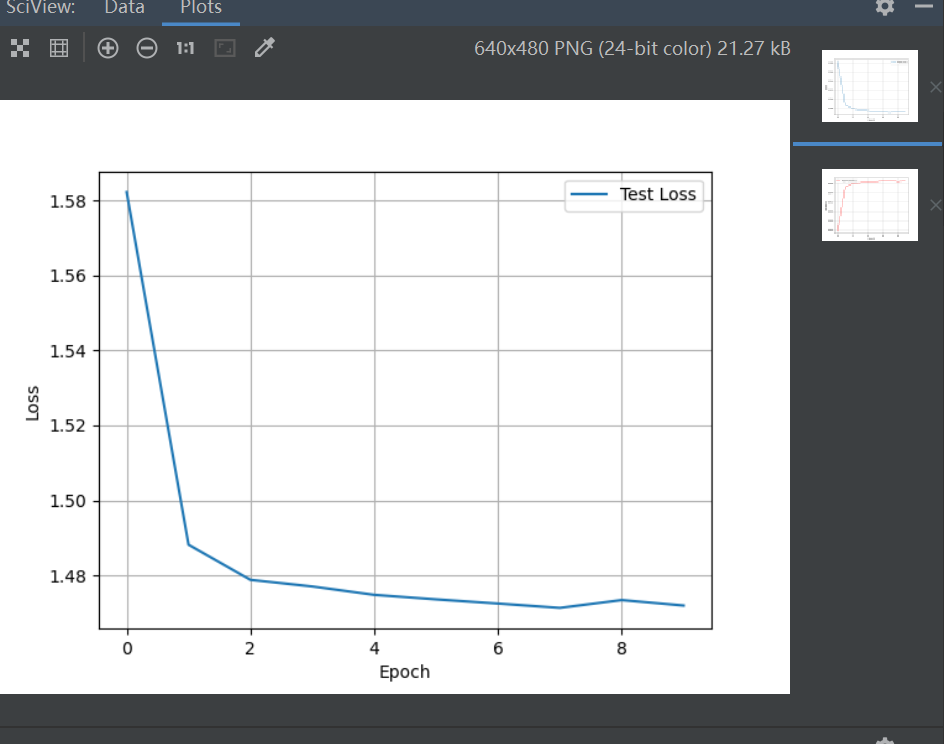
\includegraphics[width=30em]{result1.png}
%\label
\caption{test figure}
\end{figure}




\begin{table}
\centering
\caption{test table}
\begin{tabular}{p{15.1em}|lr|lr}
\hline
name & class &id\\
\hline
zhangsan & 1 & 0001\\
\hline

\end{tabular}

\end{table}

%\begin{algorithm}
%\caption{test-algorithm}
%\begin{algorithmic}
%\State Initialize parameters
%\%For {every epoch}:
%\State Do process a.
%\If{ a = 3}
%  \State Do copy a to b
%\Else if{a=5}
%  \State Remove a.
%\Endif
%\EndFor
%\end{algorithm}

\end{document}